\section{Durchführung}
\label{sec:Durchführung}

Der schematische Aufbau des Versuchs befindet sich in \autoref{fig:2}. Links 
ist der He-Ne-Laser zu sehen. Mittig liegt der Polarisationsfilter, welcher
nach Belieben eingestellt werden kann. Rechts liegt der Spiegel, welcher auf
auf einem Drehteller mit Winkelskala manifestiert ist. Daran wiederum ist der 
Detektor befestigt, welcher die Intensität am Amperemeter ausgibt.
\begin{figure}[H]
    \caption{Aufbau.}
    \centering
    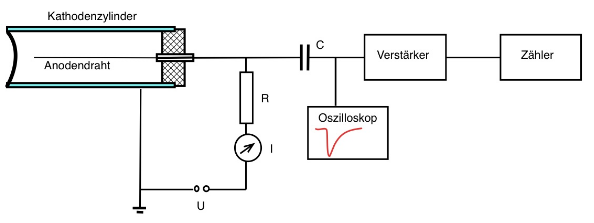
\includegraphics[width=0.7\textwidth]{"Bilder/aufbau.jpg"}
    \label{fig:2}
\end{figure}
\noindent Der Spiegel wird auf gleicher vertikaler Höhe eingestellt und der Drehteller 
mit dem Spiegel horizontal um einen Winkel von 3° ausgerichtet, das Photoelement 
wird so ausgerichtet, dass der reflektierte Lichtstrahl vom Spiegel mit 
maximaler Intensität eintrifft.
Zu Beginn wird eine Nullmessung ohne Polarisationsfilter durchgeführt um
mögliche dadurch bedingte Störfaktoren herauszufiltern. Anschließend wird 
für die senkrechte Polarisation in 2°-Schritten von 3° bis 85° der Winkel
verändert und die Intensität gemessen. Für die parallele Polarisation wird 
ebenfalls in 2°-Schritten die Intensität detektiert, allerdings wird diese 
Schrittweite präziser mit 1°-Schritten im Bereich von 69° bis 83° durchgeführt 
um den Verlauf der Intensität um den Brewster-Winkel besser nachvollziehen zu 
können.